% $Id: 20041109.tex 367 2004-11-23 10:22:38Z conall $

\documentclass[a4paper,12pt]{article}

\usepackage{graphicx}

\setlength{\parindent}{0mm}
\setlength{\parskip}{7.5mm}

\begin{document}

\title{Course 3BA5: Computer Engineering \\ Assingment 2 \\ Pipelining
Techniques in the \\ IBM PowerPC 970 (A.K.A PowerPC G5)}

\author{Conall O'Brien \\ conallob@maths.tcd.ie \\ 01734351}

\maketitle

\begin{figure}[hb]

\begin{center}

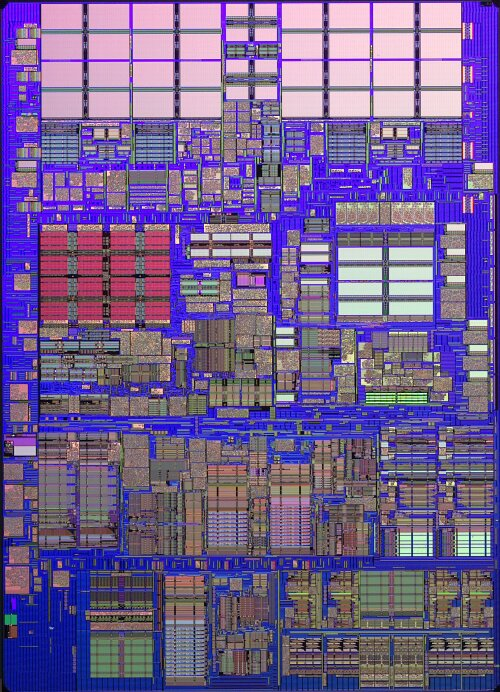
\includegraphics{powerpc970-1.png}

\end{center}

\caption{\cite[The IBM PowerPC 970 Microprocessor Unit]{a10}}

\end{figure}

\tableofcontents

\section{Overview}

The PowerPC 970 is the most recent member to the AIM (Apple, IBM,
Motorola) Consortium's PowerPC architecture commonly found in many 
systems, such as Apple Macintosh computers and various high 
performance systems. One major difference between the PowerPC 970 and other 
members of the PowerPC architecture family is it's 64 bit design, 
giving it significant 64 bit based benefits which include an 
increased memory addressing beyond the 32bit CPU limit of 4GB and 
the reduction of steps when computing high precision computations 
using multiple registers for single operands, as explained
\cite[here]{a6}

The PowerPC 970 has been designed primarily for high performance
workstation and computation roles, 

\begin{figure}[hb]

\begin{center}

\scalebox{0.5}{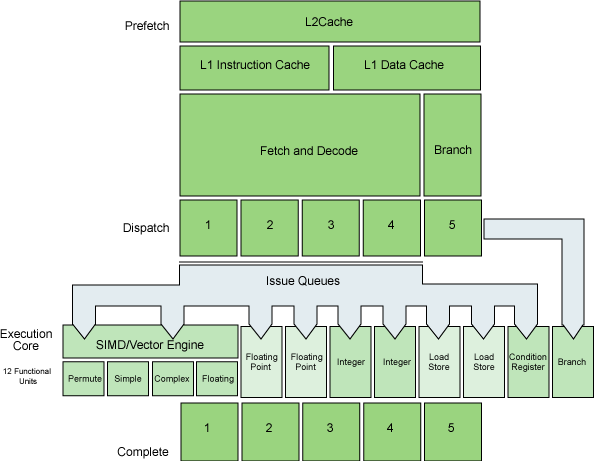
\includegraphics{970-arch.png}}

\end{center}

\caption{\cite[The IBM PowerPC 970 Microprocessor Design Layout]{a6}}

\end{figure}

\section{The Pipeline}

\subsection{Main Pipeline}

As discussed in \cite[this article]{a2}, the PowerPC 970 has 9 seperate
execution cores, including twin floating point cores, a sophisticated,
multi execution core vector processing unit, dual integer units as well
as load/store, conditional register and branch units. Combined with this
wide execution core, is a long pipeline with over 
\cite[100 execution slots]{a1}, forming a wide and deep pipeline with
mixed results.


Such a wide and deep pipeline has a few positive and negative features.
The main one being that the PowerPC 970 is capable of very high
performance computing as a result of the deep pipeline, yet it is also
flexible enough for many workstation uses with it's wide execution core.
However, in practice, such a pipeline will rarely be optimally used and
will likely include occasional pipeline stalls when converting from wide
pipelined tasks to narrow pipelined tasks in a short timeframe.

\subsection{Integer Unit}

As \cite[discussed in detail]{a2}, the Integer Units in the PowerPC 970 are not
completely symmetric, thus conditional logic is used to ensure 
most integer operations are handled by one core and integer division 
and SPR operations are handled by special hardware when required.


As a result, the Integer performance of the PowerPC 970 is less than desirable
in situations requiring frequent complex operations. Both integer units
feature 64 bit registers, so in the future when pure 64 bit software is
more common, the full potential of native 64 bit compatable integer
registers will be unleased, however, at present, very few non custom
written, high performance software utilises this feature of the integer
units of the PowerPC 970.
 
\subsection{Floating Point Unit}

With \cite[80 registers, (32 PowerPC architectural registers and 48
rename registers)]{a2} in both of the PowerPC 970's floating point units, the
floating point execution core is completely pipelined for all floating
point operations bar floating division. 


Another \cite[well renoweded feature]{a5} of the PowerPC 970's floating
point functionality is it's ability to perform a "fused multiply-add"
operation, allowing the multiplication of two floating point numbers and
the addition of a third floating point number combined in a single
opcode operaton. Although this operation is quite specialised and not
commonly utilised except using highly optimised machine code, the resulting
performance saves additional branch and arithmetic operations. 


Yet \cite[another key feature]{a2} the PowerPC 970 floating point execution core 
has the availabity to perform certain floating point operations in
hardware decoding, without the need to decode such operations into
internal PowerPC RISC based architecture opcodes.


Due to the highly regarded reputation of the recent PowerPC family
members, particularly the PowerPC 7xxx series (also called the PowerPC
G4, primarily by Apple) prior to the PowerPC 970 series, the PowerPC 
CPU line has gained a well deserved name 
for floating point performance. The fully 64 bit pipeline of both 
floating point execution units in the PowerPC 970 and the ability to fuse 
floating point multiplication and addition of floating point numbers in 
one operation greatly enhance the floating point operation performance as 
well as the already well established reputation of the floating point high 
performance. 

\subsection{Vector Unit}



\section{Conclusions}

\bibliographystyle{ieeetr}

\bibliography{PowerPC970}

\end{document}
